% Template for Cogsci submission with R Markdown

% Stuff changed from original Markdown PLOS Template
\documentclass[10pt, letterpaper]{article}

\usepackage{cogsci}
\usepackage{pslatex}
\usepackage{float}
\usepackage{caption}

% amsmath package, useful for mathematical formulas
\usepackage{amsmath}

% amssymb package, useful for mathematical symbols
\usepackage{amssymb}

% hyperref package, useful for hyperlinks
\usepackage{hyperref}

% graphicx package, useful for including eps and pdf graphics
% include graphics with the command \includegraphics
\usepackage{graphicx}

% Sweave(-like)
\usepackage{fancyvrb}
\DefineVerbatimEnvironment{Sinput}{Verbatim}{fontshape=sl}
\DefineVerbatimEnvironment{Soutput}{Verbatim}{}
\DefineVerbatimEnvironment{Scode}{Verbatim}{fontshape=sl}
\newenvironment{Schunk}{}{}
\DefineVerbatimEnvironment{Code}{Verbatim}{}
\DefineVerbatimEnvironment{CodeInput}{Verbatim}{fontshape=sl}
\DefineVerbatimEnvironment{CodeOutput}{Verbatim}{}
\newenvironment{CodeChunk}{}{}

% cite package, to clean up citations in the main text. Do not remove.
\usepackage{apacite}

% KM added 1/4/18 to allow control of blind submission
\cogscifinalcopy

\usepackage{color}

% Use doublespacing - comment out for single spacing
%\usepackage{setspace}
%\doublespacing


% % Text layout
% \topmargin 0.0cm
% \oddsidemargin 0.5cm
% \evensidemargin 0.5cm
% \textwidth 16cm
% \textheight 21cm

\title{Dimensions of Moral Status}


\author{{\large \bf Matan Mazor (mtnmzor@ucl.ac.uk)}  \AND {\large \bf Arianna Risoli (arianna.risoli.18@ucl.ac.uk)} \AND {\large \bf Anna Eberhardt (anna.everhardt.18@ucl.ac.uk)} \AND {\large \bf Stephen M. Fleming (stephen.fleming@ucl.ac.uk)} \\ University College London, \\ London WC1N 3BG}


\begin{document}

\maketitle

\begin{abstract}
Here we asked which mental and physical attributes contribute most to
decisions about moral status and the presence of consciousness in
non-human beings. Participants placed moral value on mental capacities
more than physical similarity to humans. Specifically, experimental
indications of rich and complex visual experience had strong effects on
both consciousness ratings and moral worth judgments, more so than
indications of self-awareness. Furthermore, moral worth judgments were
highly correlated with consciousness ratings, across items and
participants.

\textbf{Keywords:}
ethics; animal consciousness; meta-science
\end{abstract}

\begin{quote}
\emph{``Mama, Mama, don't kill the chicken anymore, she laid an egg! she
cares about us!''}
\end{quote}

\begin{quote}
\begin{quote}
(\emph{``Una gallina''}, Clarice Lispector, 1960)
\end{quote}
\end{quote}

\hypertarget{introduction}{%
\section{Introduction}\label{introduction}}

According to the Stanford Encyclopedia of Philosophy, an entity has
\emph{Moral Status} if and only if ``it or its interests morally matter
to some degree for the entity's own sake'' (Jaworska \& Tannenbaum,
2013). The attribution of moral status to a being affects how their
interests are taken into account in everyday decision making. For
example, the choice not to eat meat is often motivated by an attribution
of non-trivial moral status to farm animals. But how do we decide which
entities are worthy of a higher moral status, or, conversely, which can
be exploited and harmed without concern for their interests?

Philosophers have long debated which factors should be taken into
account when determining the moral status of agents. Utilitarian
philosophers Jeremy Bentham (1789) and John Stuart Mill (1861) attached
moral status to the capacity to suffer, or to sentience more generally.
Contemporary philosophical writings about the origins of moral status
debate the extent to which they should be based in private, qualitative
experience, or rather in functional or behavioural features which can be
observed by others and scientifically quantified (Carruthers, 2019;
Danaher, 2020; Levy, 2014). Crucially, regardless of what the normative
answer to this question is, in actual moral decision-making we only have
access to the behaviour of other agents, and need to infer their
internal states from these third-person observations. In other words,
regardless of whether moral status \emph{should} be based on behaviour
or experience, in practice it \emph{must} be based on behaviour, because
we can never directly perceive the subjective experience of others.

In psychology, behavioural observations are commonly used to learn about
internal mental processes, which are often assumed to have an
experiential nature for the subject. In comparative psychology, clever
experimental manipulations allow scientists to deduce latent mental
variables from observable behaviour. The mirror mark test is one such
manipulation, in which an animal's response to an unfamiliar mark on its
own reflection in the mirror is taken as a measure of self-awareness - a
mental property that cannot be directly observed (Gallup Jr, Anderson,
\& Shillito, 2002). Other known examples are the study of caching
behaviour as a measure of episodic memory (Clayton \& Dickinson, 1998)
and the use of trace-conditioning as a measure of conscious perception
(Clark, Manns, \& Squire, 2002). In all of the above examples,
scientists explain an observable behaviour as emerging from an internal
mental state.

Here we asked whether, like scientists, a random sample of online
participants would also use these and similar behaviours as indicating
the presence of mental states. We then asked whether these inferences
about conscious mental states would bias participants' moral decision
making. Our experimental design is largely based on previous studies
looking at moral status of non-human entities. Specifically, we followed
the imaginary aliens cover story used in Piazza \& Loughnan (2016), and
a moral decision-making paradigm similar to the one developed by Wilks,
Caviola, Kahane, \& Bloom (2020).

\hypertarget{experiment-1}{%
\section{Experiment 1}\label{experiment-1}}

\hypertarget{methods}{%
\subsection{Methods}\label{methods}}

Participants were presented with a story about a scientific mission to a
distant planet. According to the story, scientists have discovered
several alien species on the planet, which all have two eyes and
hand-like limbs, and all feed on space berries that grow on the planet.
The scientists sorted the alien species into 8 pairs. Within each such
pair, the two species were identical except for two differences. The
experiment then consisted of descriptions of the 8 animal pairs,
followed by questions. For each pair, participants were asked to
describe in their own words the main difference between the two alien
species. This allowed us to monitor the clarity of the descriptions and
participants' attention. Then, participants were told that a fire
started on the planet, and that two groups of aliens were caught in the
fire, one of each species. We asked the participants which group they
would rather save, assuming that the other group will die in the fire.
Lastly, participants were asked to use two sliders to indicate the
extent to which they thought each species was conscious.

For the fire dilemma, the number of aliens in the feature-positive group
(see below) was always 10. We determined the number of aliens in the
feature-negative group based on the moral decisions of previous
participants, following a Markov Chain Monte Carlo with People procedure
(Sanborn \& Griffiths, 2008). Specifically, 5 chains of 10 participants
completed the experiment. Within each chain, the first participant
decided between two groups of 10 aliens for all dimensions. In case the
participant decided to save the feature-positive group, the number of
feature-negative aliens was increased by 1 for the next participant in
the chain. In case they decided to save the feature-negative group, the
number of feature-negative aliens was decreased by 1 for the next
participants in the chain. The same rule was then followed for all 10
participants in the chain.

Within each pair, the aliens varied along one of the following
dimensions of interest: phenomenal richness, evaluative richness, unity,
temporality, selfhood, size, physical resemblance to humans in
appearance, and biological resemblance to humans. The first 5 dimensions
are based on a taxonomy of animal consciousness, described in Birch,
Schnell, \& Clayton (2020). The \emph{feature-positive} species had more
of the mental capacity of interest, or resembled humans more, compared
with the \emph{feature-negative} species. Each dimension was presented
as two scientific findings, followed by their interpretation by the
scientists, and was accompanied by cartoon figures of the experimental
design. The findings and their interpretations were based on real animal
studies. Importantly, in order not to bias participants' perception of
the aliens, the figures did not show the aliens. Alien species were
given one-syllable gibberish names, counterbalanced across participants.
Below we describe the 8 dimensions and their experimental
operationzaliations, based on animal studies. The full descriptions as
presented to our subjects are available at
\href{https://github.com/matanmazor/dimensions_of_moral_status}{github.com/matanmazor/dimensions\_of\_moral\_status}.

\begin{enumerate}
\def\labelenumi{\arabic{enumi}.}
\item
  \emph{Phenomenal Richness:} Phenomenal richness is roughly defined as
  the `level of detail with which {[}animals{]} consciously perceive
  aspects of their environment' (Birch et al., 2020). Phenomenal
  richness can vary between different sensory modalities, but for our
  study we focused on phenomenal richness in visual experience. We used
  fine-grained discrimination learning (Pearce, Esber, George, \&
  Haselgrove, 2008) and trace-conditioning (Clark et al., 2002) as our
  two operationalizations of phenomenal richness.
\item
  \emph{Evaluative Richness:} Evaluative richness is to valence what
  phenomenal richness is to sense data. It is roughly defined as the
  ability to evaluate small changes in valence and to engage in complex
  affect-based decision-making (Birch et al., 2020). We used affective
  bias (Reimert, Fong, Rodenburg, \& Bolhuis, 2017) and motivational
  trade-off (Balasko \& Cabanac, 1998) as our operationalizations of
  evaluative richness.
\item
  \emph{Unity:} Unity is roughly defined as having a ``single, unified
  perspective as opposed to multiple perspectives'' (Birch et al.,
  2020). We used interocular transfer (Ortega, Stoppa, Güntürkün, \&
  Troje, 2008) and crossmodal integration (Narins, Grabul, Soma,
  Gaucher, \& Hödl, 2005) as our two measures of unity.
\item
  \emph{Temporality:} Temporality is roughly defined as having an
  integrated stream of experience, as opposed to ``a staccato series of
  fragmented experiences'' (Birch et al., 2020). Temporality can be
  defined over short and long time scales. Here we focused on future
  planning over longer time scales (days). We used two future-planning
  paradigms (Hillemann, Bugnyar, Kotrschal, \& Wascher, 2014; Kabadayi
  \& Osvath, 2017), as our operationalizations of temporality.
\item
  \emph{Selfhood:} Selfhood is ``the conscious awareness of oneself as
  distinct from the world outside'' (Birch et al., 2020). We used the
  mirror-mark test (Gallup Jr et al., 2002) and experience projection
  (De Waal, 1986) as our two operationalizations of selfhood.
\item
  \emph{Size:} One alien species was described as having average weight
  and height of 45kg and 120cm, while the other was smaller and had
  average weight and height of 1 gram and 1 cm.
\item
  \emph{Physical resemblance to humans:} One alien species was described
  as having right and left eyes, and two hand-like limbs. The other
  alien species had upper and lower eyes, and 5 hand-like limbs.
\item
  \emph{Biological resemblance to humans:} One alien species was
  described as having red blood, and DNA that is composed of the same
  four bases as human DNA. The other alien species was described as
  having yellow blood, and DNA that is composed of entirely different
  bases.
\end{enumerate}

\hypertarget{results}{%
\subsection{Results}\label{results}}

A total of 50 participants took part in the experiment, in 5 chains of
10 participants each. Participants provided meaningful descriptions of
the different dimensions. All recorded responses, including verbal
descriptions, are openly available on
\href{https://github.com/matanmazor/dimensions_of_moral_status}{github.com/matanmazor/dimensions\_of\_moral\_status}.

\hypertarget{consciousness-ratings}{%
\subsection{Consciousness ratings}\label{consciousness-ratings}}

Participants reported the degree to which they believed the different
alien species to be conscious, on a scale of 1 to 100. Overall,
consciousness ratings were high, with a distinctive peak at the maximum
rating of 100 (mean rating = 75.90). Feature-positive species were
perceived as substantially more conscious than feature-negative species
(\(M = 8.62\), 95\% CI \([5.77\), \(11.46]\), \(t(49) = 6.09\),
\(p < .001\); see Fig. 2, upper panel). This difference in consciousness
ratings was significant for the dimensions phenomenal richness
(\(M = 10.14\), 95\% CI \([5.24\), \(15.04]\), \(t(49) = 4.16\),
\(p < .001\)), unity (\(M = 10.14\), 95\% CI \([5.24\), \(15.04]\),
\(t(49) = 4.16\), \(p < .001\)), temporality (\(M = 10.14\), 95\% CI
\([5.24\), \(15.04]\), \(t(49) = 4.16\), \(p < .001\)), and selfhood
(\(M = 17.24\), 95\% CI \([9.56\), \(24.92]\), \(t(49) = 4.51\),
\(p < .001\)). Interestingly, the perceived consciousness was also
higher for aliens with more, compared to less, biological resemblance to
humans (\(M = 9.88\), 95\% CI \([4.43\), \(15.33]\), \(t(49) = 3.64\),
\(p = .001\)). These effects survived a Bonferroni correction for our 8
manipulated variables. The effects for evaluative richness and size were
significant but did not survive correction for multiple comparisons.

\hypertarget{moral-judgments}{%
\subsection{Moral judgments}\label{moral-judgments}}

For each dimension, participants decided whether they would rather save
aliens from the feature-negative or the feature-positive species. The
number of feature-positive aliens (\(N^+\)) was always set to 10, and
the number of feature-negative aliens (\(N^-\)) followed staircase
determined by the moral judgments of previous participants -- decreasing
after decisions to save the feature-negative aliens, and increasing
following decisions to save the feature-positive aliens. We ran 5 short
(10 participant) chains in an attempt to validate our method and
establish a directional effect for our dimensions of interest. The
chains are unlikely to have converged after 10 participants, so we
refrain from interpreting our results as reflecting a true `conversion
rate' between feature-positive and feature-negative aliens.

\begin{CodeChunk}
\begin{figure}[H]

{\centering 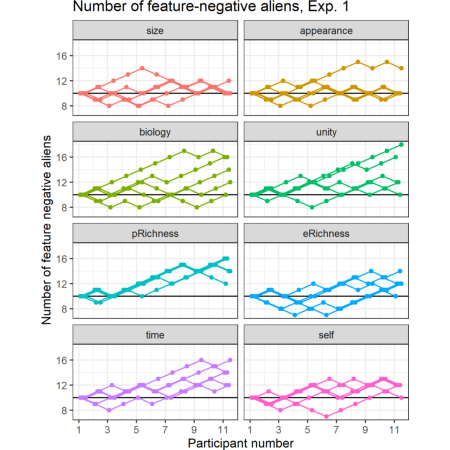
\includegraphics{figs/mwjplot1-1} 

}

\caption[The number of feature-negative aliens for each dimension as a function of participant number]{The number of feature-negative aliens for each dimension as a function of participant number. Showing data from all 5 chains. Participant number goes from 1 to 11, because the data of participant 10 dictates the number of aliens for participant 11.}\label{fig:mwjplot1}
\end{figure}
\end{CodeChunk}

We focused on the average value of \(N^-\) at the end of the chain. This
value was equal or higher than 10 for all dimensions (see Fig. 1).
Specifically, it was 14.40 for phenomenal richness, 12.00 for evaluative
richness, 13.60 for temporality and 13.60 for unity. Paralleling the
effect of biological resemblance to humans on consciousness, aliens that
were biologically similar to humans were also more likely to be saved
from the fire (\(N^-\)=13.60). If our participants were only considering
the number of aliens in each group, without any consistent effect of the
manipulated dimensions, we would expect \(N^-\) to be exactly 10 by the
10th participant. This was the case in four out of five chains for the
appearance and size dimensions. As a more conservative null model, we
simulated data from a cohort of participants that take into account the
number of aliens in each group, but not their descriptions, on 80\% of
the trials, and choose randomly on the other 20\% of the trials. The
average \(N^-\) for the last participant exceeded 11 (or went below 9)
only on 0.35\% of our 10,000 simulations, and never exceeded 12. Hence,
our empirical data provided strong evidence against this conservative
null-effect model for all 5 dimensions of consciousness, as well as for
biological resemblance to humans. In the last section of our analysis,
we asked whether beliefs about consciousness systematically covary with
biases in moral decision making.

\hypertarget{the-relation-between-moral-judgments-and-consciousness-ratings}{%
\subsection{The relation between moral judgments and consciousness
ratings}\label{the-relation-between-moral-judgments-and-consciousness-ratings}}

So far we have shown that in our data, inference about the presence of
consciousness in imaginary aliens was informed by descriptions of
behaviours which are interpreted in the scientific literature on animal
consciousness as signs of phenomenal richness, evaluative richness,
unity, temporality, and selfhood (Birch et al., 2020), as well as by
beliefs about their biological resemblance to humans. We also showed
that the same factors contributed to moral judgments about these
imaginary aliens. Our experimental design is not optimized to test for a
causal link between these two findings. However, we can quantify the
extent to which variability in beliefs about consciousness explains
variability in judgments of moral status.

Across dimensions, high values of \(N^-\) were associated with a more
pronounced difference between consciousness ratings for the
feature-positive and feature-negative alien species (see Fig. 4). One
exception was selfhood, scoring highest in consciousness ratings (with a
mean difference of 18.75 between feature-positive and feature-negative
aliens), but having only moderate effects on moral status judgments
(\(N^-\)=11.6). In Experiment 2 we look closer at the two
operationalizations of selfhood in our study, mirror self recognition
and deception, and ask whether this mismatch between consciousness
ratings and moral worth judgments is common to both.

Unlike size and resemblance to humans in physical appearance, biological
resemblance to humans (operationalized as the color of aliens' blood and
the building blocks that make up their genetic code), had strong effects
on moral status judgments and on beliefs about the presence of
consciousness. This was the only physical dimension that showed these
effects. In order to test if the effect on moral status judgments was
related to the effect on consciousness ratings, we contrasted the
difference in consciousness ratings between feature-positive and
feature-negative species as a function of participants' decision to save
the feature-positive or the feature-negative group. A difference would
indicate that those participants who saved the feature-positive group
also thought they tended to be more conscious. Note that this test
marginalizes over different values of \(N^-\). Indeed, the difference in
consciousness ratings was lower in those participants who chose to save
the feature-negative group (\(\Delta M = -14.11\), 95\% CI \([-21.26\),
\(-6.95]\), \(t(38.00) = -3.99\), \(p < .001\)).

\hypertarget{experiment-2}{%
\section{Experiment 2}\label{experiment-2}}

In Experiment 1, we found that short descriptions of scientific findings
affected participants' attribution of consciousness to imaginary aliens
as well as their moral status judgments. We also found evidence for a
relation between these two effects, reflected in the alignment of
consciousness ratings and moral status judgments, across subjects and
dimensions. One exception to this alignment was the selfhood dimension,
where a strong effect on the attribution of consciousness did not
translate to a strong effect on moral status judgments. Finally, while
size and physical appearance had no effect on the attribution of
consciousness and moral status judgments, biological resemblance to
humans had strong effects on both. In Experiment 2, we zero in on these
effects and focus on the dimensions of selfhood, biological resemblance
to humans, phenomenal richness, and physical resemblance to humans in
appearance.

\hypertarget{methods-1}{%
\subsection{Methods}\label{methods-1}}

Experiment 2 followed a similar procedure to Experiment 1, except for a
few differences. First, each alien pair corresponded to a single
scientific observation: mirror self-recognition (Gallup Jr et al.,
2002), capacity for deception (De Waal, 1986), blood color, DNA building
blocks, discrimination learning (Pearce et al., 2008), trace
conditioning (Clark et al., 2002), eye position and number of limbs.
Second, participants were not given information about the way scientists
interpreted the findings. Third, to simplify and shorten the experiment,
we simplified some of the descriptions, and omitted all figures.
Finally, in order to allow the MCMC chains to converge, we ran two
chains of 110 participants each.

\hypertarget{results-1}{%
\subsection{Results}\label{results-1}}

A total of 220 participants took part in the experiment, in 2 chains of
110 participants each. Participants provided meaningful descriptions of
the different dimensions. All recorded responses, including verbal
descriptions, are openly available on
\href{https://github.com/matanmazor/dimensions_of_moral_status}{github.com/matanmazor/dimensions\_of\_moral\_status}.

\hypertarget{consciousness-ratings-1}{%
\subsection{Consciousness ratings}\label{consciousness-ratings-1}}

Participants reported the degree to which they believed the different
alien species were conscious, on a scale of 1 to 100. Overall,
consciousness ratings were high, with a distinctive peak at the maximum
rating of 100 (mean rating = 71.91). Feature-positive species were
perceived as substantially more conscious than feature-negative species
(\(M = 8.53\), 95\% CI \([6.58\), \(10.48]\), \(t(216) = 8.60\),
\(p < .001\)). This difference in consciousness ratings was significant
for all features except for the number of limbs. These effects survived
a Bonferroni correction, except for the effect for blood colour.

\begin{CodeChunk}
\begin{figure}[H]

{\centering 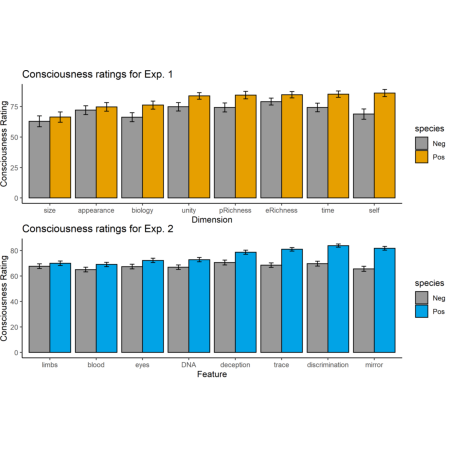
\includegraphics{figs/consciousness_plot2-1} 

}

\caption[Consciousness ratings for the eight species pairs in Experiment 1]{Consciousness ratings for the eight species pairs in Experiment 1. Participants attributed more consciousness to feature-positive aliens. }\label{fig:consciousness_plot2}
\end{figure}
\end{CodeChunk}

\hypertarget{moral-judgments-1}{%
\subsection{Moral judgments}\label{moral-judgments-1}}

Similar to experiment 1, participants decided whether they would rather
save aliens from the feature-negative or the feature-positive species.
Here also, the number of feature-positive aliens (\(N^+\)) was always
set to 10, and the number of feature-negative aliens (\(N^-\)) followed
the moral judgments of previous participants. Longer chains allowed us
to estimate the conversion rate between feature-positive and
feature-negative aliens for each of our eight features. We discarded the
first 10 \(N^-\) values as a burn-in period, and took the mean of the
remaining 101 values as our estimate for \(N^-\). Generally, we observed
high levels of agreement between the two chains (see Fig. 3). One
exception was mirror recognition, with mean \(N^-\) of 13.63 and 11.48
for chains number 1 and 2.

In line with the results from Experiment 1, \(N^-\) was highest for
discrimination learning (16.16) and trace conditioning (14.65), both
operationalizations of the phenomenal richness dimension from Exp. 1. In
other words, participants valued the lives of aliens who showed signs of
visual phenomenal richness about 1.5 more than the lives of aliens who
did not show these signs. Next, mirror self-recognition had moral value
(\(N^-=\) 12.56, but see above comment about convergence), whereas the
capacity to deceive others, also typically taken as a sign of
self-awareness, had a neutral moral value (\(N^-=\) 9.71). This was the
case even though participants saw it as a reliable sign of consciousness
(mean difference in consciousness ratings for deceivers and
non-deceivers: \(M = 8.14\), 95\% CI \([4.02\), \(12.26]\)).
Participants also attributed greater value to the lives of aliens whose
DNA was composed of the same DNA bases as human DNA (\(N^-=\) 12.17).
Finally, eye configuration (\(N^-=\) 11.05), the colour of the blood
(\(N^-=\) 10.88), and the number of limbs (\(N^-=\) 10.06), all had only
small to negligible effects on moral judgments.

\begin{CodeChunk}
\begin{figure}[H]

{\centering 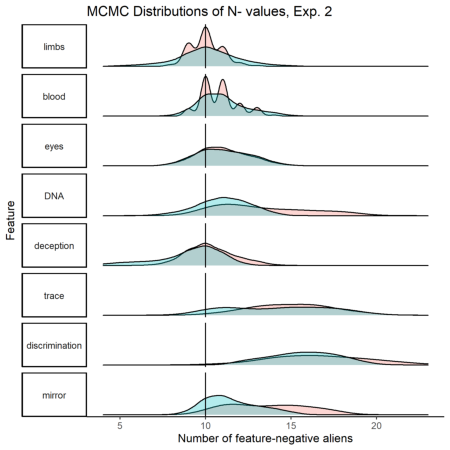
\includegraphics{figs/mwjplot2-1} 

}

\caption[Distributions of N- values for the two MCMC chains (red and blue)]{Distributions of N- values for the two MCMC chains (red and blue). All features but mirror-recognition showed high levels of convergence between the two chains.}\label{fig:mwjplot2}
\end{figure}
\end{CodeChunk}

\hypertarget{the-relation-between-moral-judgments-and-consciousness-ratings-1}{%
\subsection{The relation between moral judgments and consciousness
ratings}\label{the-relation-between-moral-judgments-and-consciousness-ratings-1}}

Consciousness ratings were strongly aligned with \(N^-\) across features
(see Fig. 4). This alignment is remarkable, as consciousness ratings
were reported on a 1-100 scale by individual participants, while \(N^-\)
was extracted from binary decisions of many participants. Similar to
Experiment 1, this linear alignment held for all features except for the
selfhood-related ones: mirror self-recognition and capacity for
deception. Finally, in agreement with our results from Experiment 1,
participants who chose to save aliens who were more biologically similar
to humans (operationalized as blood color, or DNA building blocks), also
perceived those aliens to be more conscious (blood:
\(\Delta M = -8.88\), 95\% CI \([-13.71\), \(-4.05]\),
\(t(140.59) = -3.64\), \(p < .001\), DNA: \(\Delta M = -11.18\), 95\% CI
\([-16.29\), \(-6.07]\), \(t(215.37) = -4.31\), \(p < .001\)),
suggesting that the effect of biological similarity to humans on moral
status was tightly linked with, and potentially causally mediated by,
beliefs about consciousness.

\begin{CodeChunk}
\begin{figure}[H]

{\centering 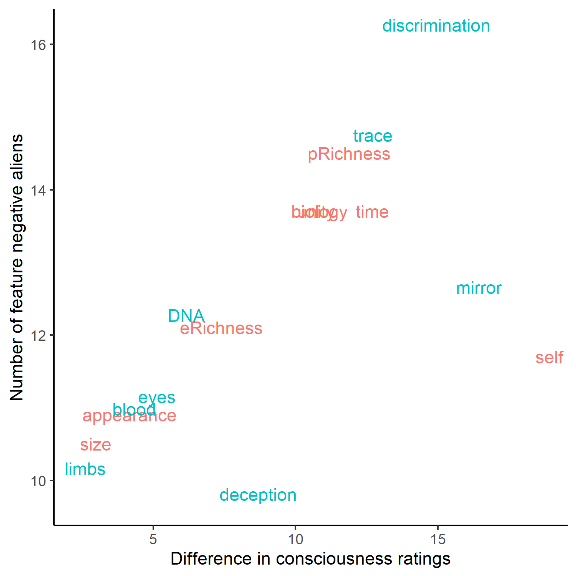
\includegraphics{figs/relation_scatter-1} 

}

\caption[Association between moral status judgments and consciousness attribution for our 8 dimensions of Experiment 1 (red) and the 8 features of Experiment 2 (cyan)]{Association between moral status judgments and consciousness attribution for our 8 dimensions of Experiment 1 (red) and the 8 features of Experiment 2 (cyan). Self-related attributes were shifted from the diagonal, with a strong effect on consciousness ratings that did not translate to a strong effect on moral decision making.}\label{fig:relation_scatter}
\end{figure}
\end{CodeChunk}

\hypertarget{discussion}{%
\section{Discussion}\label{discussion}}

In two experiments, participants made moral judgments about the life and
death of imaginary aliens. Using imaginary aliens allowed us to
experimentally manipulate beliefs about abstract dimensions (Experiment
1) or specific features (Experiment 2), and measure their causal effect
on moral decision making and beliefs about conscious experience. Both
consciousness ratings and moral decisions were sensitive to our
manipulation. Specifically, consciousness ratings were affected more by
our five dimensions of consciousness (phenomenal and evaluative
richness, unity, temporality, and selfhood, based on a taxonomy by Birch
et al., 2020) than by physical attributes such as biological or physical
similarity to humans. Furthermore, we found that dimensions of conscious
experience had a substantial effect on participants' moral decisions.
One exception was selfhood and its constituent operationalizations
mirror self recognition and capacity for deception, which had only weak
effects on moral judgments despite having strong effects on
consciousness ratings.

Previous work has established a strong relation between moral decision
making and the ascription of mental attributes such as intelligence,
experience, or agency. For example, beliefs about the capacity for
subjective experience were associated with a desire to avoid harm (Gray,
Gray, \& Wegner, 2007). Similarly, being told that an animal or an alien
is more intelligent made participants more likely to report that it was
not OK to eat them (Piazza \& Loughnan, 2016), and this association
between perceived intelligence and moral worth was apparent already in
young children (Wilks et al., 2020). We build and extend on these
findings in two ways. First, adopting a fine-grained taxonomy of
dimensions of conscious experience (Birch et al., 2020) revealed
different effects for different dimensions on moral status. Second,
Experiment 2 provided evidence that people extract information about
conscious experience from behavioural observations, similar to the
interpretation of behavioural findings by comparative psychologists, and
that they use this information to guide their moral decision making.
This second finding is especially important in light of the debates over
the moral significance of functional versus phenomenal aspects of
consciousness (Carruthers, 2019; Danaher, 2020; Levy, 2014).

In both experiments we found a strong alignment between consciousness
ratings and moral status, with the single exception of selfhood and its
constituent operationalizations, which contributed to consciousness
ratings much more than to moral status (see Fig. 4). While we are not
aware of any study that directly examined the effects of perceived self
awareness on moral status, the idea that moral worth is based on
self-awareness dates back at least to Emmanuel Kant (1785). In a
striking contrast with this notion, here we find that beliefs about
lower-level aspects of consciousness such as visual awareness and
working memory are much more influential for moral decision-making than
beliefs about selfhood, more in line with the utilitarian views of Mill
(1789) and Bentham (1861), and more recently with the view of Shepherd
(2018).

\hypertarget{acknowledgements}{%
\section{Acknowledgements}\label{acknowledgements}}

\hypertarget{references}{%
\section{References}\label{references}}

\setlength{\parindent}{-0.1in} 
\setlength{\leftskip}{0.125in}

\noindent

\hypertarget{refs}{}
\leavevmode\hypertarget{ref-balasko_motivational_1998}{}%
Balasko, M., \& Cabanac, M. (1998). Motivational conflict among water
need, palatability, and cold discomfort in rats. \emph{Physiology \&
Behavior}, \emph{65}(1), 35--41.
\url{http://doi.org/10.1016/S0031-9384(98)00090-0}

\leavevmode\hypertarget{ref-bentham1789utilitarian}{}%
Bentham, J. (1789). A utilitarian view. \emph{Animal Rights and Human
Obligations}, 25--26.

\leavevmode\hypertarget{ref-birch2020dimensions}{}%
Birch, J., Schnell, A. K., \& Clayton, N. S. (2020). Dimensions of
animal consciousness. \emph{Trends in Cognitive Sciences}.

\leavevmode\hypertarget{ref-carruthers2019human}{}%
Carruthers, P. (2019). \emph{Human and animal minds: The consciousness
questions laid to rest}. Oxford University Press.

\leavevmode\hypertarget{ref-clark2002classical}{}%
Clark, R. E., Manns, J. R., \& Squire, L. R. (2002). Classical
conditioning, awareness, and brain systems. \emph{Trends in Cognitive
Sciences}, \emph{6}(12), 524--531.

\leavevmode\hypertarget{ref-clayton1998episodic}{}%
Clayton, N. S., \& Dickinson, A. (1998). Episodic-like memory during
cache recovery by scrub jays. \emph{Nature}, \emph{395}(6699), 272--274.

\leavevmode\hypertarget{ref-danaher2020welcoming}{}%
Danaher, J. (2020). Welcoming robots into the moral circle: A defence of
ethical behaviourism. \emph{Science and Engineering Ethics},
\emph{26}(4), 2023--2049.

\leavevmode\hypertarget{ref-de1986deception}{}%
De Waal, F. (1986). Deception in the natural communication of
chimpanzees. \emph{Deception: Perspectives on Human and Nonhuman
Deceit}, 221--244.

\leavevmode\hypertarget{ref-gallup2002mirror}{}%
Gallup Jr, G. G., Anderson, J. R., \& Shillito, D. J. (2002). The mirror
test. \emph{The Cognitive Animal: Empirical and Theoretical Perspectives
on Animal Cognition}, 325--333.

\leavevmode\hypertarget{ref-gray2007dimensions}{}%
Gray, H. M., Gray, K., \& Wegner, D. M. (2007). Dimensions of mind
perception. \emph{Science}, \emph{315}(5812), 619--619.

\leavevmode\hypertarget{ref-hillemann2014waiting}{}%
Hillemann, F., Bugnyar, T., Kotrschal, K., \& Wascher, C. A. (2014).
Waiting for better, not for more: Corvids respond to quality in two
delay maintenance tasks. \emph{Animal Behaviour}, \emph{90}, 1--10.

\leavevmode\hypertarget{ref-jaworska2013grounds}{}%
Jaworska, A., \& Tannenbaum, J. (2013). The grounds of moral status.

\leavevmode\hypertarget{ref-kabadayi2017ravens}{}%
Kabadayi, C., \& Osvath, M. (2017). Ravens parallel great apes in
flexible planning for tool-use and bartering. \emph{Science},
\emph{357}(6347), 202--204.

\leavevmode\hypertarget{ref-kant1785moral}{}%
Kant, I. (1785). \emph{The moral law: Groundwork of the metaphysic of
morals}.

\leavevmode\hypertarget{ref-levy2014value}{}%
Levy, N. (2014). The value of consciousness. \emph{Journal of
Consciousness Studies}, \emph{21}(1-2), 127--138.

\leavevmode\hypertarget{ref-mill1861utilitarianism}{}%
Mill, J. S. (1861). Utilitarianism.

\leavevmode\hypertarget{ref-narins2005cross}{}%
Narins, P. M., Grabul, D. S., Soma, K. K., Gaucher, P., \& Hödl, W.
(2005). Cross-modal integration in a dart-poison frog. \emph{Proceedings
of the National Academy of Sciences}, \emph{102}(7), 2425--2429.

\leavevmode\hypertarget{ref-ortega2008limits}{}%
Ortega, L. J., Stoppa, K., Güntürkün, O., \& Troje, N. F. (2008). Limits
of intraocular and interocular transfer in pigeons. \emph{Behavioural
Brain Research}, \emph{193}(1), 69--78.

\leavevmode\hypertarget{ref-pearce2008nature}{}%
Pearce, J. M., Esber, G. R., George, D. N., \& Haselgrove, M. (2008).
The nature of discrimination learning in pigeons. \emph{Learning \&
Behavior}, \emph{36}(3), 188--199.

\leavevmode\hypertarget{ref-piazza2016meat}{}%
Piazza, J., \& Loughnan, S. (2016). When meat gets personal, animals'
minds matter less: Motivated use of intelligence information in
judgments of moral standing. \emph{Social Psychological and Personality
Science}, \emph{7}(8), 867--874.

\leavevmode\hypertarget{ref-reimert2017emotional}{}%
Reimert, I., Fong, S., Rodenburg, T. B., \& Bolhuis, J. E. (2017).
Emotional states and emotional contagion in pigs after exposure to a
positive and negative treatment. \emph{Applied Animal Behaviour
Science}, \emph{193}, 37--42.

\leavevmode\hypertarget{ref-sanborn2008markov}{}%
Sanborn, A., \& Griffiths, T. L. (2008). Markov chain monte carlo with
people. In \emph{Advances in neural information processing systems} (pp.
1265--1272).

\leavevmode\hypertarget{ref-shepherd2018consciousness}{}%
Shepherd, J. (2018). \emph{Consciousness and moral status}. Taylor \&
Francis.

\leavevmode\hypertarget{ref-wilks2020children}{}%
Wilks, M., Caviola, L., Kahane, G., \& Bloom, P. (2020). Children
prioritize humans over animals less than adults do. \emph{Psychological
Science}, 0956797620960398.

\bibliographystyle{apacite}


\end{document}
